\section[Neutronové zdroje]{Měření základních charakteristik radionuklidových, generátorových a fotoneutronových zdrojů neutronů}
Asi bych to všechno měřil v manganové lázni, ale to asi nebude úplně oukej :D\footnote{Tím změříš jenom emisivitu, jinak je ti to k prdu :D}.

Zdroje neutronů jsou významným nástrojem  ve vědeckých, výzkumných, lékařských, ale i přírodních a průmyslových aplikací. Nejvíce využívanými zdroji pro tyto obory jsou výzkumné jaderné reaktory, které poskytují dostatečně vysoké hustoty toku neutronů, ovšem jejich nevýhodou jsou vysoké pořizovací a provozní náklady.

\subsection{Radionuklidové zdroje}

Pokud není vyžadována vysoká intenzita, lze využít tzv. radionuklidové zdroj. Jejich výhodou jsou malé rozměry, snadná přeprava, nízké nároky na údržbu, jednoduchá obslužnost a nízká cena.

Jedním ze zástupců radionuklidového zdroje je AmBe zdroj. Americium je $\alpha$ zářič, který emituje jádra $^4_2$He s poločasem rozpadu $T_{1/2}= 433,6$ let. Jádra helia jsou zachycena na beryliu za vzniku uhlíku a volného neutronu:

\begin{equation*}
    ^{9}\text{Be} + ^{4}\text{He} \longrightarrow  ^{12}\text{C} + ^1_0\text{n}.
\end{equation*}

Energie uvolněného neutronu se pohybuje okolo $10\ $MeV.

Radionuklidový zdroj bych měřil v manganové lázni. Podrobně zpracováno jnde.

\subsection{Generátorové zdroje}

Generátory neutronů jsou kompaktní zařízení, které produkují neutrony na základě fúzní reakce dvou izotopů vodíku. Fúzní reakce probíhá pomocí urychlených částic D nebo T v terči z kovového hydridu (D, T nebo směs). 

\begin{align*}
^2\text{H} + ^2\text{H} &\to ^3\text{He} + \text{n}, & Q &= 3.27 \, \text{MeV}, \\
^3\text{H} + ^3\text{H} &\to ^4\text{He} + 2\text{n}, & Q &= 11.33 \, \text{MeV}, \\
^2\text{H} + ^3\text{H} &\to ^4\text{He} + \text{n}, & Q &= 17.59 \, \text{MeV}.
\end{align*}

Fúzní reakce probíhá pomocí urychlených částic D nebo T v terči z kovového hydridu.

Generátory neutronů jsou obvykle kompaktní a přenosné přístroje. Využívají reakce D-D, T-T nebo D-T, což umožňuje jejich široké použití. Výstup neutronů se pohybuje v rozmezí od $10^6$ n/s do $10^{11}$ n/s. Při vyšších výtěžcích je nutné zajistit chlazení terče. Tyto generátory mohou pracovat v kontinuálním nebo pulzním režimu. Frekvence jejich provozu může být od jednotek Hz až po desítky kHz, přičemž šířka jednotlivých pulzů dosahuje až desítek $\mu$s. Emise neutronů je řízena počítačem, což zajišťuje přesnost a kontrolu nad provozem zařízení.

Na Obrázek \ref{fig:Schéma neutronového generátoru} je zobrazeno schéma neutronového generátoru.

\begin{figure}[H] 
    \centering
    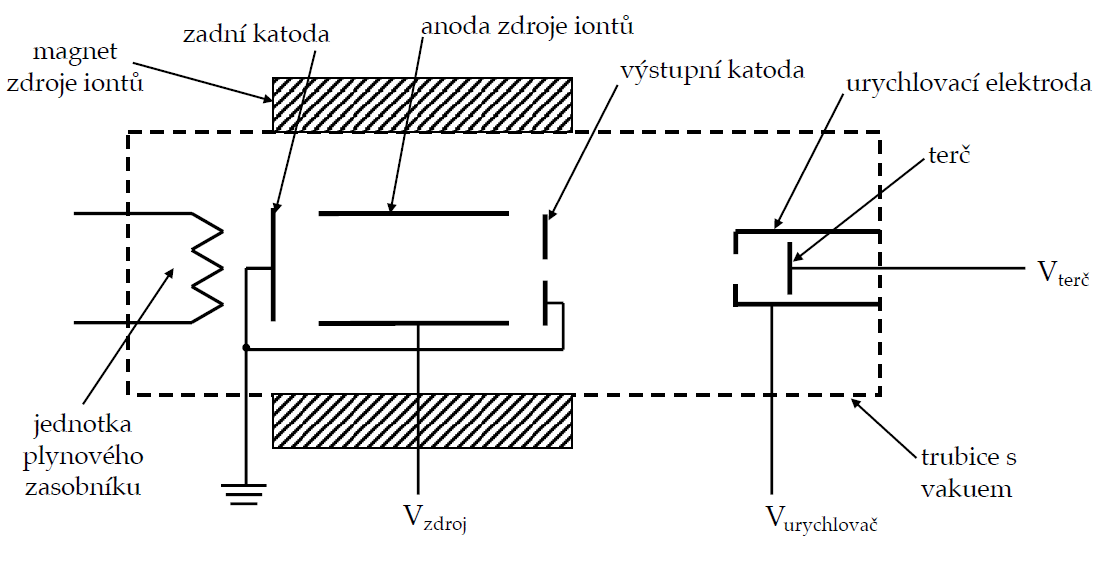
\includegraphics[scale=0.49]{img/generator.png}
    \caption{Schéma neutronového generátoru.}
    \label{fig:Schéma neutronového generátoru}
\end{figure}

\begin{figure}[H] 
    \centering
    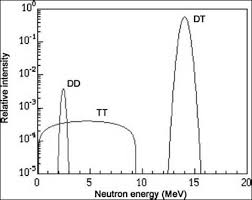
\includegraphics[scale=1.0]{img/SpektrumNeutronůZFůzníhoGenerátoru.jpg}
    \caption{Spektrum neutronů produkovaných fúzními generátory neutronů.}
    \label{fig:SpektrumNeutronůZFůzníhoGenerátoru}
\end{figure}


\subsection{Fotonoutronové zdroje}

Foton dopadající na jádro může způsobit vyražení neutronu z jádra v případě, že jeho energie je větší než energie, se kterou je neutron vázán v jádře. Vhodnými zdroji fotonů jsou radioaktivní prvky, které však emitují gama kvanta, jejichž energie je obvykle nižší než prahová energie reakce. Z tohoto důvodu jsou pro foto-neutronové reakce optimální terčová jádra s nižší prahovou energií (viz Tabulka \ref{tab:fotoneutronove_reakce}). Nejčastěji jsou jako terčový materiál využívána jádra $^2$H a $^9$Be. Typickým představitelem foto-neutronového zdroje, který je v praxi využíván, je zdroj typu $^{124}$SbBe. 

S foto-neutrony se můžeme setkat při provozu jak energetických (těžkovodní reaktory typu CANDU), tak i výzkumných reaktorů (výzkumné reaktory, které používají beryllium nebo těžkou vodu).

Hlavní výhodou foto-neutronových zdrojů je, že v případě použití mono-energetického gama záření jsou emitované neutrony také mono-energetické a jejich energie je oproti tradičním radionuklidovým zdrojům neutronů výrazně nižší (řádově od desítek až po několik stovek keV). Naproti tomu nevýhodami jsou nízký výtěžek neutronů a obtíže spojené s přítomností vysokoenergetického gama záření o značné intenzitě.

Gama kvanta vysokých energií i intenzity lze také získat použitím různých typů urychlovačů částic. V jejich případě nejsou produkovány mono-energetické neutrony, jelikož tato zařízení poskytují gama kvanta větší spektrální šíře.

\begin{table}[h!]
\centering
\caption{Přehled vybraných terčových nuklidů používaných pro foto-neutronové reakce.}
\label{tab:fotoneutronove_reakce}
\begin{tabular}{ccc}
\toprule
\textbf{Terčový nuklid} & \textbf{Prahová energie (MeV)} & \textbf{Reakce} \\ \midrule
$^2\text{H}$            & 2,225                         & $^2\text{H}(\gamma, n)^1\text{H}$ \\ 
$^6\text{Li}$           & 3,697                         & $^6\text{Li}(\gamma, n + p)^4\text{He}$ \\ 
$^6\text{Li}$           & 5,670                         & $^6\text{Li}(\gamma, n)^5\text{Li}$ \\ 
$^7\text{Li}$           & 7,251                         & $^7\text{Li}(\gamma, n)^6\text{Li}$ \\ 
$^9\text{Be}$           & 1,667                         & $^9\text{Be}(\gamma, n)^8\text{Be}$ \\ 
$^{13}\text{C}$         & 4,900                         & $^{13}\text{C}(\gamma, n)^{12}\text{C}$ \\ \bottomrule
\end{tabular}

\end{table}

\subsubsection{Foto-neutronové reakce}

Nejběžnějšími foto-neutronovými reakcemi jsou reakce záření gama s jádry beryllia a deuteria:

\begin{align*}
    \text{Be}^9 + \gamma & \rightarrow \text{Be}^8 + n, \\
    \text{H}^2 + \gamma & \rightarrow \text{H}^1 + n.
\end{align*}

Jedná se o endotermické reakce s prahovou energií $1.63$~MeV v případě beryllia a $2.18$~MeV u deuteria. Vzhledem k endotermické povaze těchto reakcí, budou mono-energetické fotony produkovat mono-energetické neutrony. Ze zákona zachování energie a hybnosti můžeme odvodit vztah pro energii foto-neutronu:

\begin{equation}
E_n = \frac{A - 1}{A} \cdot \left[ E_\gamma - Q - \frac{E_\gamma^2}{1862 \cdot (A - 1)} \right] + \delta
\end{equation}

kde:

\begin{itemize}
    \item $E_n$ -- je energie neutronu (MeV),
    \item $A$ -- je hmotnostní číslo terčového jádra,
    \item $E_\gamma$ -- je energie gama záření (MeV),
    \item $Q$ -- je prahová energie (energie reakce) pro ($\gamma$, n) reakci.
\end{itemize}

$\delta$ je malý rozptyl energie, který je funkcí úhlu $\theta$ mezi dopadajícím gama kvantem a emisí neutronu a lze jej popsat vztahem:

\begin{equation}
\delta = E_\gamma \cdot \left[ \frac{2 \cdot (A - 1) \cdot (E_\gamma - Q)}{931 \cdot A^3} \right]^2 \cdot \cos \theta
\end{equation}

\begin{table}[h!]
\centering
\caption{Parametry vybraných radioizotopů včetně poločasu rozpadu ($T_{1/2}$), energie gama záření ($E_\gamma$) a intenzity gama záření ($I_\gamma$).}
\label{tab:radioizotopy}
\begin{tabular}{cccc}
\toprule
\textbf{Radioizotop} & \boldmath$T_{1/2}$ & \boldmath$E_\gamma$ \textbf{(MeV)} & \boldmath$I_\gamma$ \textbf{(\%)} \\ \midrule
$^{24}\text{Na}$     & 14,96 h           & 2,75                               & 99,94                             \\ 
$^{28}\text{Al}$     & 2,24 m            & 1,78                               & 100                               \\ 
$^{38}\text{Cl}$     & 37,24 m           & 1,64; 2,17                         & 31,9; 42,4                        \\ 
$^{56}\text{Mn}$     & 2,58 h            & 1,81; 2,11                         & 27,2; 14,3                        \\ 
$^{116m}\text{In}$   & 54,29 m           & 1,75; 2,11                         & 2,46; 15,5                        \\ 
$^{124}\text{Sb}$    & 60,20 d           & 1,69; 2,09                         & 47,79; 5,51                       \\ \bottomrule
\end{tabular}
\end{table}

Radioizotopy s poločasem kratším než jedna hodina nejsou obvykle využívány pro fotoneutronové zdroje, jelikož jejich životnost je příliš krátká. Pro experimentální práce s tímto typem zdrojů je nutné, aby jejich poločas rozpadu byl alespoň několik hodin nebo spíše několik dnů. 

Aby příslušný fotoneutronový zdroj byl monoenergetickým zdrojem neutronů, musí používaný radionuklid vyzařovat gama kvanta pouze s jednou energií nad prahem reakce.


\subsubsection{Vlastnosti foto-neutronových zdrojů}

Mezi základní charakteristiky fotoneutronových zdrojů patří energie a výtěžek neutronů. Důležitým parametrem je také životnost takového zdroje, která je dána poločasem rozpadu gama zářiče.

Charakteristické energie neutronů pro reakce různých zdrojů gama záření s deuteriem a berylliem jsou uvedeny v Tabulce~\ref{tab:fotoneutrony_energie}.

\begin{table}[h!]
\centering
\caption{Energie fotoneutronů pro různé reakce ($\gamma$, n).}
\label{tab:fotoneutrony_energie}
\begin{tabular}{@{}lc@{}}
\toprule
\textbf{Reakce}       & \boldmath$E_n$ \textbf{(MeV)} \\ \midrule
$^{24}\text{Na} + \text{Be}$ & 1,00                         \\
$^{24}\text{Na} + \text{D}$  & 0,29                         \\
$^{28}\text{Al} + \text{Be}$ & 0,15                         \\
$^{38}\text{Cl} + \text{Be}$ & 0,46; 0,0187                 \\
$^{56}\text{Mn} + \text{Be}$ & 0,15; 0,45                   \\
$^{56}\text{Mn} + \text{D}$  & 0,26                         \\
$^{116m}\text{In} + \text{Be}$ & 0,15; 0,46                 \\
$^{124}\text{Sb} + \text{Be}$ & 0,060; 0,42                 \\ \bottomrule
\end{tabular}
\end{table}

\begin{table}[h!]
\centering
\begin{tabular}{@{}lc@{}}
\toprule
\textbf{Reakce}       & \textbf{Výtěžek neutronů (s\textsuperscript{-1})} \\ \midrule
$^{24}\text{Na} + \text{Be}$ & $14 \cdot 10^4$ \\
$^{24}\text{Na} + \text{D}_2\text{O}$  & $29 \cdot 10^4$ \\
$^{56}\text{Mn} + \text{Be}$ & $2,9 \cdot 10^4$ \\
$^{56}\text{Mn} + \text{D}_2\text{O}$  & $0,31 \cdot 10^4$ \\
$^{116m}\text{In} + \text{Be}$ & $0,82 \cdot 10^4$ \\
$^{124}\text{Sb} + \text{Be}$ & $19 \cdot 10^4$ \\ \bottomrule
\end{tabular}
\caption{Výtěžek neutronů pro různé reakce ($\gamma$, n) a zdroj gama záření o aktivitě 1 Ci.}
\label{tab:vytezky_neutronu}
\end{table}
